\documentclass[a4paper,10pt,twocolumn]{article}

\usepackage{graphicx}
\begin{document}
\title{\emph{BlkKin}: An end-to-end tracing tool for software defined storage 
systems}
\date{}
\maketitle

\section*{Abstract}
Distributed storage systems require special treatment concerning their
monitoring and tracing. The need for production scale live tracing arises since
under these circumstances, interesting and problematic behaviors are most likely
to become obvious. However, this need in conjunction with low-latency and
high-throughput demands set further challenges, apart from the initial ones
concerning distributed tracing like clock synchronization and trace correlation.

In this paper we describe the development of a low-impact, live tracing
infrastructure used in monitoring large scale storage systems. \emph{BlkKin} is
a system based on LTTng\cite{lttng}, implementing the tracing schema proposed in
the Dapper paper\cite{dapper}. We have successfully used \emph{blkin} in a
software defined storage system called Archipelago\cite{archip} and  backed by
RADOS\cite{rados}. We traced and measured IO requests initiated within the VMs
until they were finally served by RADOS.


\textbf{Keywords: } tracing, monitoring, low-latency, LTTng, RADOS

\section{Introduction}

The more complex the distributed systems are becoming today, the greater grows
the need for better debugging and monitoring tools. However, debugging or
monitoring a distributed system is a difficult and demanding job. Dealing with
multiple hosts makes the system's behavior unpredictable and bound to a specific
context that could change from execution to execution. Thus, finding failures or
bottlenecks cannot be achieved through traditional performance analysis or
debugging tools. 

This problem can be tackled through tracing. Tracing captures the state of the
system along with other needed information that could provide further insight of
the exact context that a specific event happened. These information can be
correlated to explore the system's behavior under different working states.
Unlike traditional monitoring that could be achieved out of the box, in order to
obtain, this kind of information, instrumentation points should be placed in the
system's source code indicating the events to be traced and the values to be
measured.

Tracing a distributed system can be very challenging and various problems may
arise. In order for the tracing to be valuable, the system should be traced
under real working conditions, since most of the failures are about to appear at
full load. So, ideally we would like to have a fully functional system working
at production scale that is getting traced at the same time. So, the tracing
mechanism should not affect the system's performance significantly. Also, since
we want to explore a distributed system's behavior, we have to deal with
multiple hosts and events happening almost simultaneously. This sets two
different challenges. How to qualitatively correlate event information and how
to quantitatively correlate time information between different hosts. For the
first problem, a certain mechanism should group together all the traces
concerning a specific initial request. For the second problem, since we approach
performance analysis as well, the tracing mechanism should handle the time
differences between the hosts' clocks and try to eliminate them. These
differences may be crucial when analyzing time latencies.

Some of the most widespread distributed systems are the distributed storage
systems. These systems can be used either as huge data warehouses for images,
videos etc, or as storage backends for virtual volume provisioning employed by
IAAS providers. In any case, their performance analysis and tuning is of vital
importance since large latencies may end up to an unresponsive system and user
dissatisfaction.

In this paper, we present the design and implementation of \emph{BlkKin}.
\emph{BlkKing} is a system that enables us to debug and monitor through tracing
a distributed storage system in real time, with a very low overhead and
visualize the aggregated information. This information, coming from cross-layer
tracing, enables us to explore the system's behavior under various circumstances
and workloads, since we have at our disposal an accurate, end-to-end
representation of the request's route from the time it enters the system till it
is finally served revealing time latencies between the different layers and the
possible bottlenecks that our system may have. In order to fulfil the previous
prerequisites, we make use of \emph{LTTng} (Linux Trace Toolkit - next
generation)\cite{lttng} for low overhead tracing and the tracing schema used in
Google's Dapper for tracing information correlation.

As a use-case, we are using \emph{BlkKin} in tracing a software defined storage
system \emph{Archipelago}\cite{archip}. Archipelago is used by Synnefo
\cite{synnefo}, an IAAS provider software and uses RADOS\cite{rados} as storage
backend. Consequently, with \emph{BlkKin} we trace the IO requests from the time
they are created within the VM, till they are finally served by RADOS.

\section{Tracing logic} One of the most important aspects of system tracing is
the aggregated information correlation and interpretation. There are two
dominant schools concerning tracing information interpretation. \emph{Black box}
monitoring scheme assumes there is no additional information other than the
message record. So statistical regression techniques should be used to infer any
existent association. \emph{Annotation-based} schemes, on the other hand, rely
on applications or middleware to explicitly tag every record with a global
identifier that links these message records back to the originating request. In
order to have an overall review of the system per specific request, we have to
implement an annotation-based monitoring scheme.

In order to capture the information needed for the end-to-end tracing, our
tracing schema should be able firstly to group all the traces belonging to the
same request and secondly depict the causal relationships between the different
layers, taking into account that the system is distributed, thus providing
information about the hosts. Also, it should enable us to collect any other
information considered important, by though custom data annotations.

Google proposed a complete annotation-based monitoring scheme in the Dapper
paper\cite{dapper}. This proposed scheme meets our mentioned demands and was
chosen to used in \emph{BlkKin}. In short, Dapper describes the following
semantics for tracing:
\begin{description}
\item[annotation]
The actual information being logged. There are two kinds of annotations. Either
\emph{timestamp}, where the specific timestamp of an event is being logged or 
\emph{key-value}, where a specific key-value pair is being logged.
\item[span]
The basic unit of the process tree. Each specific processing phase can be 
depicted as a different span. Each span should have a specific name and a 
distinct span id.
\item[trace]
Every span is associated with a specific trace. A different trace id is used to
group data so that all spans associated with the same initial request share the
common trace id. For our case, information concerning a specific IO request
share the same trace id and each distinct IO request initiates a new trace id.
\item[parent span] 
In order to depict the causal relationships between different spans in a single
trace, parent span id is used. Spans without a parent span ids are  known as 
\emph{root spans}.
\end{description}

So, by creating tracing data according to these semantics we can have an
end-to-end sense of our system's performance, behavior and internal latencies
that may vary depending on the nature and size of each request that can also be
captured using key-value annotations for example.

\subsection{Logic implementation} Based on these primitives, Twitter created
Zipkin\cite{zipkin}, a distributed tracing system used to gather timing data for
all the disparate services running on their premises. Zipkin consists of a data
collector, a database service and a Web interface to visualize the aggregated
data, created according to the principles described above.

Zipkin uses Scribe\cite{scribe} to transport traces from the different services.
Scribe is a logging server created by Facebook, aiming to be scalable and
reliable. Scribe servers are arranged in a directed graph, with each server
knowing only about the next server in the graph. This network topology allows
for adding extra layers of fan-in, as a system grows and batching messages
before sending them between datacenters as well as providing reliability in case
of intermittent connectivity or node failure. Scribe makes use of
Thrift\cite{thift} for data transfer.

Zipkin seemed to fit our demands concerning data collection since it is designed
to scale. Also, the used SQL-schema was adequate to capture and query all the
needed tracing information and finally, the Web UI offered us descriptive
visualization of the traces, apart from the SQL-interface used for more
elaborate queries. Although Zipkin offers various libraries (Python, Ruby,
Scala) in order to instrument applications, there was no providence for
low-latency applications written in C/C++. Our contribution was to create a
C/C++ library that encapsulates the Dapper semantics and can be used within
C/C++ projects to create trace information in accordance with the Dapper logic.
This library is designed to be backend-independent, which means that one can
implement his own log aggregation backend for the library. However, we offered a
specific backend implementation according to our initial prerequisites
concerning overhead that is being thoroughly examined in the next chapter.

\section{Low overhead tracing} As mentioned before, a storage system's
performance is a crucial matter. Both throughput and latency should be
unaffected by tracing. So every approach to monitor or trace this kind of
systems should have the least possible added overhead to the instrumented
application which should continue working properly production-wise.

\subsection{Tracing backend} \emph{BlkKin} was designed driven by this strict
low-overhead and production-wise operation prerequisite. So the first important
decision to make concerned the system that would implement the system's backend,
namely the system that would run on every cluster node and would be responsible
for aggregating tracing data from the instrumented applications. So we chose to
use \emph{LTTng} (Linux Trace Toolkit - next generation)\cite{lttng} in our
system backend.

\emph{LTTng} is a toolchain that allows integrated kernel and user-space tracing
from a single user interface. \emph{LTTng} was initially designed and
implemented to reproduce, under tracing, problems occurring in normal
conditions. It encapsulates synchronization primitives that meet the low-impact
requirements by using a linearly scalable and wait-free RCU (Read-Copy Update)
synchronization mechanism. This mechanism was implemented in kernel and then
ported to userspace as well. In addition, \emph{LTTng} supports a variety of
operating systems (Debian, Fedora, Arch) and since version 2.x kernel tracer
modules are built against a vanilla or distribution kernel, without need for
additional patches.  So, \emph{LTTng} satisfied our prerequisites concerning
overhead and enabled us to use the same generic toolkit for both user and kernel
tracing while being easily installed on almost every system needed to
instrument. 

LTTng supports static tracepoint instrumentation. This means to manually insert
tracepoints in the application source code and rebuild the application. After
rebuilt, these tracepoints will breakpoint-less and system-call-less produce the
described traces as far as userspace is concerned. As far a kernel-space is
concerned, LTTng is supported by kprobes and kernel markers. Thus LTTng does not
significantly affect the system's performance and is ideal to operate as backend
for our C/C++ tracing library mentioned before. Although the whole process of
recompiling the instrumented application may seem counterproductive, static
instrumentation abilities are limitless. Based on the knowledge and
understanding of the application, one can instrument and trace every part that
might be problematic or causing longer latencies, as well as extracting all the
information needed to fully understand under which context each request was
served. Consequently, since since we wanted to implement the Dapper tracing
semantics, static tracing was the only way to do that.

\subsection{Live tracing} 
As mentioned before, performance tracing should happen while the system operates
in production. All the vulnerabilities, faults, or bottlenecks would become
obvious in a production environment. This would mean to trace a production
system and in real time have access and process the aggregated information,
without separating the tracing from the operating phase. Although this may sound
natural for traditional logging systems like syslog, in combination with the
demand for low-impact tracing, several difficulties arise. Older tracing
approaches required separation between the tracing and operation phases. This
happened either because tracing added a lot of extra overhead to the
instrumented system so it could not continue working production-wise, or because
tracing information was not in a state that could be processed before the end of
the tracing session. For LTTng especially, tracing data were in a binary form
that could be decoded only after the end of the tracing session. 

\subsubsection{Infrastructure} Since version 2.4 of \emph{LTTng}, live tracing
is possible. Tracing data can be streamed, decoded and processed in real time
using a daemon process called \emph{relayd} that collects the tracing data over
the network using batch TCP packets.  

However, \emph{LTTng} live tracing supports only its native CTF format.
Consequently, in order to be able to process and visualize tracing data in real
time with Zipkin, we needed to implement a live-tracing plugin that would
transform in real time CTF data to Scribe messages sent to either a local or the
central Zipkin Scribe server. So based on Babeltrace\cite{bltrace}, which is a
CTF converter and trace viewer, we developed a plugin that reads and decodes the
CTF-formatted information, it creates Thrift\cite{thrift} encoded messages
recognizable by the Zipkin collector and sends these messages to the Scribe
server. So we end up with the architecture presented in
Figure\ref{fig:specific}.

The instrumented application produces tracing information according to the
Dapper semantics using our custom made tracing library, through instrumentation
points in its source code. This information is aggregated by \emph{LTTng} and
sent to the \emph{relayd} daemon. After that, our Babeltrace plugin gets the
tracing data from the relayd, processes them as mentioned and finally sends them
to the Scribe server. 

\subsubsection{Deployment} In Figure~\ref{fig:specific} each arrow represents a
TCP communication. This offers us a lot of versatility concerning deployment.
Based on specific needs and cluster architecture each service can run on a
different node. Also, the Scriber server, that the Babeltrace plugin finally
sends the tracing information to, can be either the central Zipkin collector or
a local Scribe daemon that will eventually send the data to the central
collector, thus exploiting the asynchronous, buffered communication provided by
Scribe.

So in a cluster deployment with many nodes, we end up having the architecture
presented in Figure~\ref{fig:generic}. In this deployment, there is a whole
\emph{BlkKin} stack running on every node of the cluster. The communication
described in Figure\ref{fig:specific} takes place over localhost and the tracing
data will end up being handled by a local Scribe daemon. This daemon will
normally send the data to the cental Zipkin collector, but also store them
locally in case of a connection loss or if the central Zipkin collector is busy
and try to send them later.  So we can make sure that no data will be lost,
because any data loss would mess up the tracing semantics and end up with an
inconsistent UI and database state.

\begin{figure}[h!]
  \centering
  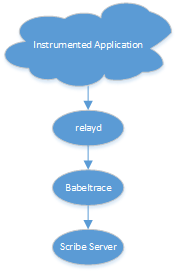
\includegraphics[scale=0.75]{images/specific.png}
  \caption{\emph{BlkKin} architecture}
  \label{fig:specific}
\end{figure}

\begin{figure}[h!]
  \centering
  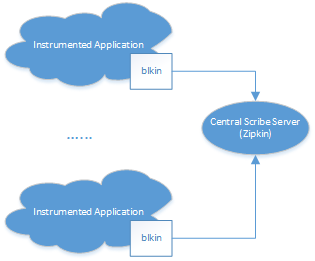
\includegraphics[scale=0.75]{images/generic.png}
  \caption{\emph{BlkKin} deployment}
  \label{fig:generic}
\end{figure}

\section{Clock Synchronization}

A crucial matter that needs special treatment when it comes to distributed
tracing is clock synchronization. In a \emph{BlkKin} cluster deployment, ideally
we would like to have no time difference between the cluster nodes' clocks,
since we are interested in measuring latencies and processing durations in the
scale of microseconds. So, a possible time skew in the scale of milliseconds
could result in having a response virtually happening before its triggering
request.

In order to solve this problem various solutions have been proposed. Before
2010, NTP's precision was within the interval from 100 $\mu$s to 2 ms. Such
precision was unacceptable for tracing storage systems. So NTP was abandoned as
a clock synchronization mechanism and instead post-tracing, statistical methods
were developed in order to adjust time differences. Time skews were approximated
using arithmetic analysis methods like linear regression. In these methods, each
node collected traces using its own clock. Afterwards, considering a specific
node as anchor, time differences from the anchor were calculated for the whole
tracing duration for all cluster nodes. For each node, these deltas where
interpolated in order to find the best approximation for the time skew
throughout the tracing session. The new approximated deltas were applied to the
collected timestamps in a separate layer, before the tracing information were
finally stored. According to \cite{hp} these methods performed well. However,
their disadvantage was the post processing overhead which could be significant
for long tracing sessions and the fact that live tracing was not possible.

However, the new version of NTP (version 4), published in June 2010, improved
NTP's synchronizing potential accuracy to the tens of microseconds with modern
workstations and fast LANs. According to our measures, with a LAN communication
time at about <?>, after <?> NTP's precision reached <?>.  So, instead of just
using the same global NTP server for all the cluster nodes, we used one single
cluster node serving as NTP server for the rest. Thus exploiting the fast LAN
interconnecting the cluster nodes, we achieved the needed accuracy.
 
\section{Evaluation - Usecase}

\begin{thebibliography}{9}
\bibitem{rados}
    RADOS: A Scalable, Reliable Storage Service for Petabyte-scale
    Storage Clusters
\bibitem{archip}
    Archipelago,
    info about
\bibitem{lttng}
    LTTng,
    info about
\bibitem{systemtap}
    SystemTap,
    info about
\bibitem{bltrace}
    Babeltracep,
    info about
\bibitem{dapper}
    Dapper,
    info about
\bibitem{zipkin}
    Zipkin,
   info about
\bibitem{scribe}
    scribe,
   info about
\bibitem{thrift}
    scribe,
   info about
\bibitem{synnefo}
    scribe,
   info about
\bibitem{hp}
    hp paper
\end{thebibliography}
\end{document}
